\documentclass{article}
\usepackage{amsmath, amssymb}
\usepackage[english]{babel}
\usepackage{fullpage}
\usepackage{graphicx}
\usepackage[hidelinks]{hyperref}
\usepackage[round,authoryear]{natbib}
\bibliographystyle{plainnat}
\usepackage{microtype}

\author{Dieuwke Hupkes}
\title{Experiments}
\date{}

\begin{document}

\maketitle

% \section{Intro}

\section{Datasets}

I define the following set of languages:

\begin{table}[!ht]
\begin{tabular}{lcl}
    \textbf{Name} & \textit{Numeric leaves} &  \textit{Example}\\
    \hline
    $L_2$ & 2  & ($x_1$ \textit{op} $x_1$)\\
    $L_3$ & 3  & (($x_1$ \textit{op} $x_2$) \textit{op} $x_3$)\\
    $L_4$ & 4  & (($x_1$ \textit{op} $x_2$) \textit{op} ($x_3$ \textit{op} $x_4$))\\
    \dots & &\\
\end{tabular}
\end{table}

\noindent Where $x_i\in\{-19,19\}$, and \textit{op} $\in\{+,-\}$. The meaning $y$ of e sentences is the result of the arithmetic expression expressed by the languag. We restrict the languages to include only expressions such that $y\in\{-60,60\}$.\\

\noindent We define the following subsets of the languages defined above:

\begin{table}[ht!]
\begin{tabular}{llll}
    \textbf{Name} & \textit{Restriction} & \textit{Example} \\
    \hline
    $L_i+$ & \textit{op} $==+$ & $(.(.(x_1 + x_2) + \dots x_i)$ & Structurally non ambiguous\\
    $L_i-$ & \textit{op} $==-$ & $(.(.(x_1 - x_2) - \dots x_i)$ &\\
    $L_i$right & only right branching trees & $(.(.(x_1$ \textit{op} $x_2)$ \textit{op} $x_3)$ \textit{op} $\ldots x_i)$ & Structurally non ambiguous\\
    $L_i$left & only left branching trees & $(x_1$ \textit{op} $(x_2$ \textit{op} ($\ldots$ \textit{op} $(x_{i-1}$ \textit{op} $x_i).).)$ & Structurally non ambiguous\\
\end{tabular}
\end{table}

The datasets that the networks will be trained and tested on are (subsets of) unions of the languages described above.

\section{Architectures}

I experiment with 2 different architectures:

\begin{figure}[!ht]
\setlength{\tabcolsep}{18pt}
\begin{tabular}{|cc|cc|}
    \hline
    \textbf{A1} & \textbf{A4} \\ % & \textbf{A3} & \textbf{A4}\\
    & \\
    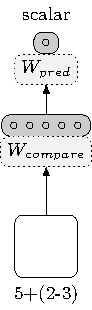
\includegraphics[scale=0.9]{A1} & 
    % 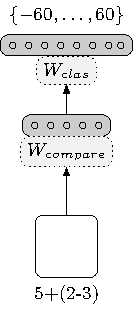
\includegraphics[scale=0.9]{A2} &
    % 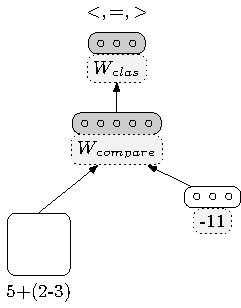
\includegraphics[scale=0.9]{A3} &
    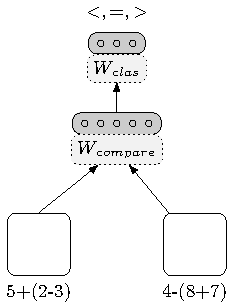
\includegraphics[scale=0.9]{A4}\\
\hline
\end{tabular}
\end{figure}

\section{Aims and questions}

There are a couple questions I would like to answer:\begin{enumerate}
\item Can a recurrent network (setup A1) learn to generalise to sentence lengths that weren't in the training set?
\item Can a recurrent network learn right branching languages (and generalise to longer phrases)
\item Can a recurrent network learn the full arithmetic language? How is the solution encoded?
\end{enumerate}

To answer these questions I should figure out what appropriate training regimes are and what the impact is of initialisation and the size of the hidden and comparison layer. Also I will need to find some methods to analyse the internal dynamics of the network (correlatie tussen activatie units oid? welke gewichten zijn hoog? eigenwaardes weights matrix?)

\section{Experiments}

\subsection{A4}

\subsubsection{Setup}

I first tested the network on the arithmetic task in a way similar to Sara. Details of the networks and training:

\begin{tabular}{ll}
    Languages train &\\
    Languages test &\\
    Size embeddings & \\
\end{tabular}


Train on 25000 examples with L1, L2, L4 and L6 expressions, validate on 2500 examples of the same languages, test on 1200 examples with L3, L5 and L7 expressions. Size hidden = 15; size compare = 2; embeddings size = 2; epochs = 800 for simpleRNN, 200 for GRU; batch size = 24; optimizer = adam; digits = -10,\dots, 10. All numbers are averages over 25 runs.\\

\begin{table}[!h]
\begin{tabular}{l|cccc|cccc|cccc}
            & \multicolumn{4}{c}{training} & \multicolumn{4}{c}{validation} & \multicolumn{4}{c}{test}\\
            & mean & min & max & std & mean & min & max & std & mean & min & max & std \\ 
\hline
SimpleRNN   & 0.93 & 0.87 & 0.95 & 0.02 & 0.92 & 0.87 & 0.95 & 0.02 & 0.59 & 0.09 & 0.94 & 0.34\\ 
GRU         & 0.97 & 0.96 & 0.97 & 0.003 & 0.96 & 0.95 & 0.97 & 0.006 & 0.94 & 0.93 & 0.95 & 0.007\\      
\end{tabular}
\end{table}

Empirical baselines: (ignore brackets)

\begin{tabular}{|l|ccc|}
    \hline
    & training & validation & test\\
simpleRNN & 0.83 & 0.51 & 0.76\\
& 0.83 & 0.83 & 0.76\\
& 0.84 & 0.83 & 0.76\\
\hline
GRU & 0.84 & 0.82 & 0.77\\
& 0.85 & 0.82 & 0.74\\
& 0.84 & 0.81 & 0.77\\
\hline
\end{tabular}


% \subsection{A1}
% 
% Note: these results are not significant, but just based on my experience with a couple runs with different settings.\\
% 
% \noindent In all my experiments I use embeddings of size 2, a comparison layer of size 2, batch size 24 and random initialisation.
% 
% \subsection{L2}
% 
% Different operators, but no structural ambiguity: finite state.\\
% 
% \noindent No gates or memory units are necessary to learn the L2 language. 
% How well and how quickly depends on the size of the hidden layer (as is to be expected).
% For 10 hidden units the results vary, training sometimes converges much quicker than other times, but in all runs I did a prediction error of at least less than 0.5 was reached.
% With 15 hidden units the network generally converges faster, and reaches a higher accuracy (although still seems quite dependent on initialisation).\\
% 
% Regardless of the accuracy, in the (2 dimensional) plots of the learned embeddings the embeddings are always on an (almost) ordered line, with the plus and minus far away from each other on different sides of the line (for an example see Figure \ref{fig:L2_embeddings}).
% 
% \begin{figure}[!ht]
%     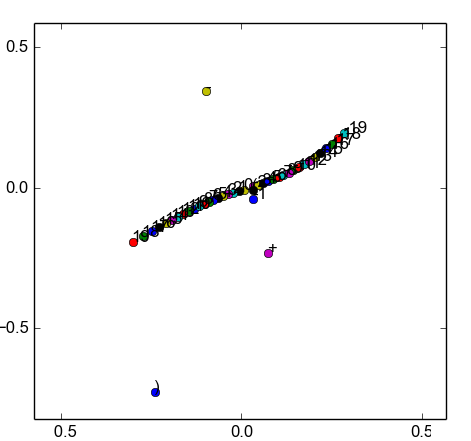
\includegraphics[scale=0.7]{L2_embeddings.png}
%     \caption{Learned embeddings for a network with 15 simple recurrent units and a comparison layer of size 2. The network was trained on 1800 L2 sentences for 5000 epochs, batch size 24. After training, the mspe of the validation set (200 different L2 sentences) was 0.01.}\label{fig:L2_embeddings}
% \end{figure}
% 
% \subsection{L+}
% 
% No structural ambiguity, but longer sentences, finite state.\\
% 
% I switched the optimizer to adam, the prediction error is more all over the place (and seems to be not entirely converged at the end of the training). 
% The network generally decreases its error at the start of the training much faster, but also finds more non generalisable solutions?
% It seems that the network is better able to generalise if longer test sequences are included in training
% 
% \begin{tabular}{lcccc}
%     trained on & mspe training & mspe test L4+ & mspe L5+ & mspe L7+\\
%     L2+, L3+, L6+ & 0.13 & 0.03 & 0.04 & 0.17\\
%     L2+, L3+, L6+ & 0.08 & 0.03 & 0.04 & 0.16\\
%     L2+, L3+, L6+ & 0.04 & 0.01 & 0.02 & 0.13\\
%     \hline
%     L2+, L3+, L4+ & \\
%     L2+, L3+, L4+ & \\
%     L2+, L3+, L4+ & \\
% \end{tabular}
% 
% I also tried to train the L+ language with dropout (0.05), that worked very poorly!
% 
% \subsection{L3}
% 
% Test if we can train on L3 and predict L2? What does the solution look like.\\
% \noindent Test if we can train on L2, L3 and L4 and predict sentences from L5\\
% \noindent Test if we can train on L2, L3 and L6 and predict sentences from L5 and L7\\
% 


\section{What will I monitor?}

I will have to think of some things I can monitor to see what it is actually doing, ideas?\begin{itemize}
    \item During training:\begin{itemize}
            \item plot the eigenvalue of the recurrent connection matrix?
            \item kleurenplaatje gewichten van input naar hidden?
        \end{itemize}
    \item While running the network:\begin{itemize}
            \item correlaties tussen hidden units?
            \item correlaties tussen input en hidden units?
            \item changeability hidden units over tijd?
            \item miss hidden layer activaties plotten voor voorbeelden?
        \end{itemize}
    \end{itemize}

\section{Comments, to do}

\begin{itemize}
    \item Currently it is not possible to check for consistency of teh map between the words in the vocabulary and integers. I should build this at some point, although I am not sure what would be a good way to do so. An option would be to modify the embeddings class and add the dmap as an attribute. Or maybe I could write my own model class that contains that, or always run models as a tuple with the dmap?
    \item it would be good to make some tests\dots
\end{itemize}



% General settings I am using for all simulations: hidden size = 20, size comparison layer = 10, batch size = 24, optimizer = adagrad.
% 
% 
% \subsection{L2}
% 
% I ran a few run with Architecture 1, size\_hidden = 20, size\_compare=10, size\_embeddings = 2 and language = L2. 
% The trainingset contains 1800 sentences, validation set contains 200 sentences, batchsize during training was 24. 
% During most runs the prediction error (= the sum squared differences between the true outcome and the rounded scalar prediction of the network) on the validation set stays high for a while and then rapidly decreases to a value close to 0. 
% Examples of learned embeddings are depicted in \ref{fig:L3_embeddings} and \ref{fig:L3_embeddings2}.
% 
% \begin{figure}[!ht]
%         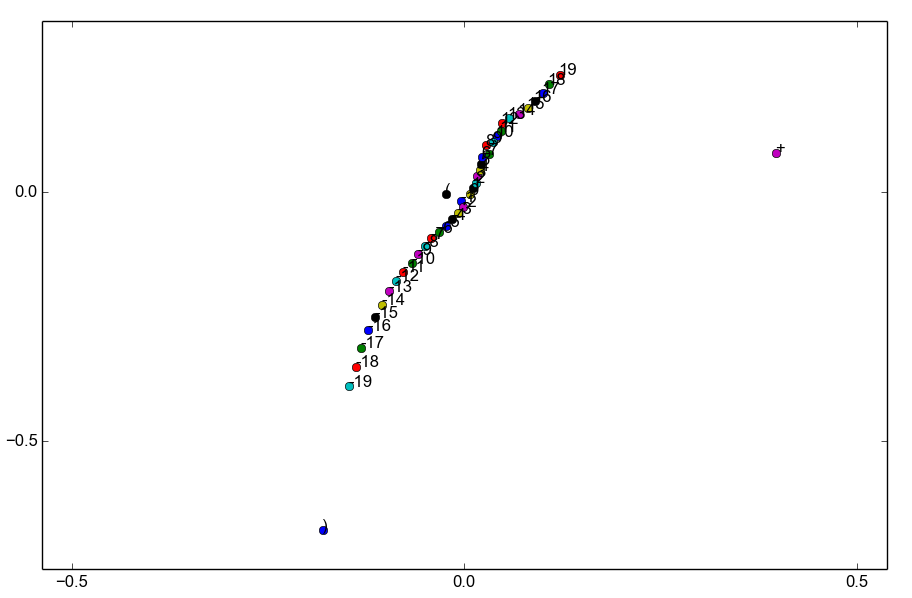
\includegraphics[scale=0.5]{L2_embeddings2.png}
%         \caption{Learned embeddings for network trained on 1800 L2 sentences and tested on 200 different L2 sentences. After 1500 epochs, the mean squared prediction error on the 200 sentences in the validation set was 0.76}\label{fig:L3_embeddings2}
% \end{figure}
% 
% \subsection{Training L+ languages SRN}
% 
% I did a couple runs with structurally unambiguous plus languages. 
% Settings of the network were still the same: size\_hidden = 20, size\_compare=10, size\_embeddings = 2. 
% I trained for 1000 epochs.\\
% 
% The numbers are still more or less ordered, but not as strongely as before. 
% The brackets and + do not get a meaningful embedding (they are both very close to 0), which is sensible because in the + languages they do not contribute to the meaning of the sentence.
% Examples of learned embeddings are shown in Figure \ref{fig:SRN_L2L3L6_testL5} and Figure \ref{fig:SRN_L2L3L4_testL5}.\\
% 
% It seems the simple recurrent network does not really learn a very general solution for the addition operator: when the sentence length of the test items is shorter than the longest training item (even though the exact length was not in the trainingset) the network performs the task with a very low training error. 
% When the sentence length is longer than the longest training item, the network does not learn to perform the task.
% 
% \begin{figure}[!ht]
%         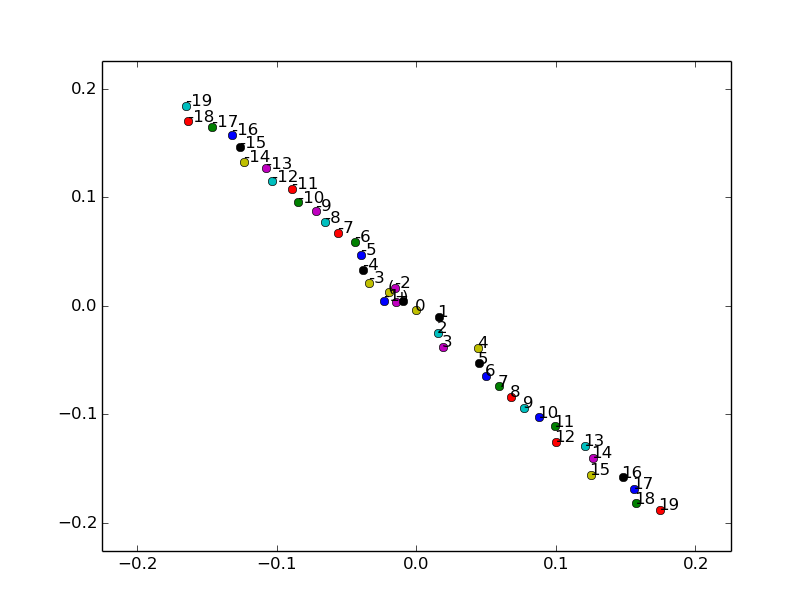
\includegraphics[scale=0.8]{SRN_L2L3L6.png}
%         \caption{Learned embeddings for SRN trained on 2000 L2+ sentences, 2000 L3+ sentences and 2000 L6+ sentences, and tested on 500 L4 sentences. After 1000 epochs, the mean squared prediction error on the 200 sentences in the validation set was 0.056}\label{fig:SRN_L2L3L6_testL5}
% \end{figure}
% 
% \begin{figure}[!ht]
%         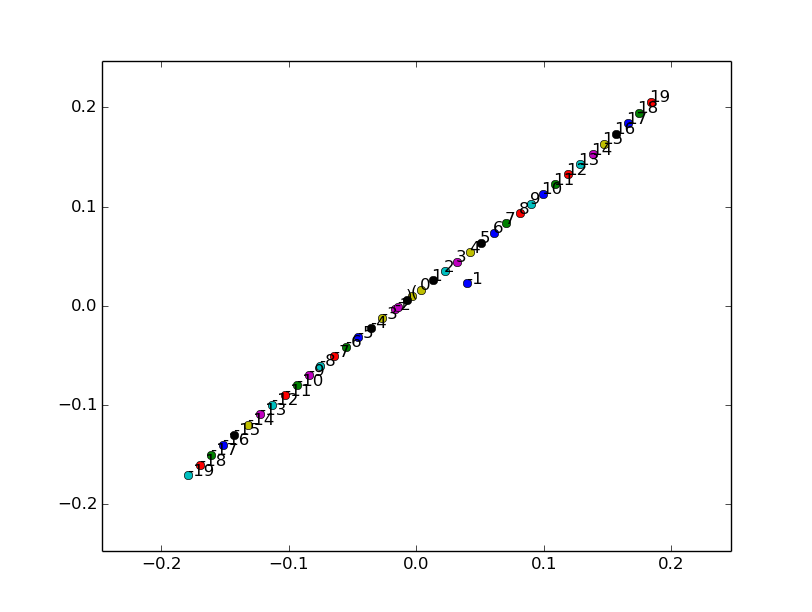
\includegraphics[scale=0.8]{SRN_L2L3L4.png}
%         \caption{Learned embeddings for SRN trained on 2000 L2+ sentences, 2000 L3+ sentences and 2000 L4+ sentences, and tested on 500 L5+ sentences. After 1000 epochs, the mean squared prediction error on the 200 sentences in the validation set was 24.1 (the mspe of the trainingset was 0.006).}\label{fig:SRN_L2L3L4_testL5}
% \end{figure}
% 
% \begin{figure}[!ht]
%         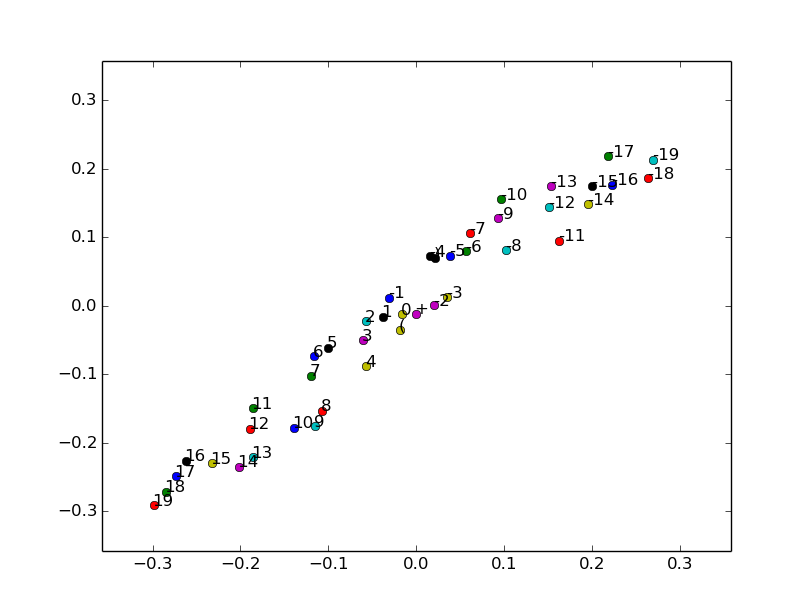
\includegraphics[scale=0.8]{GRU_L2L3L4.png}
%         \caption{Learned embeddings for network with GRU layer trained on 2000 L2+ sentences, 2000 L3+ sentences and 2000 L4+ sentences, and tested on 500 L5+ sentences. After 1000 epochs, the mean squared prediction error on the 200 sentences in the validation set was 0.04}\label{fig:GRU_L2L3L4}
% \end{figure}
% 
% \begin{figure}[!ht]
%     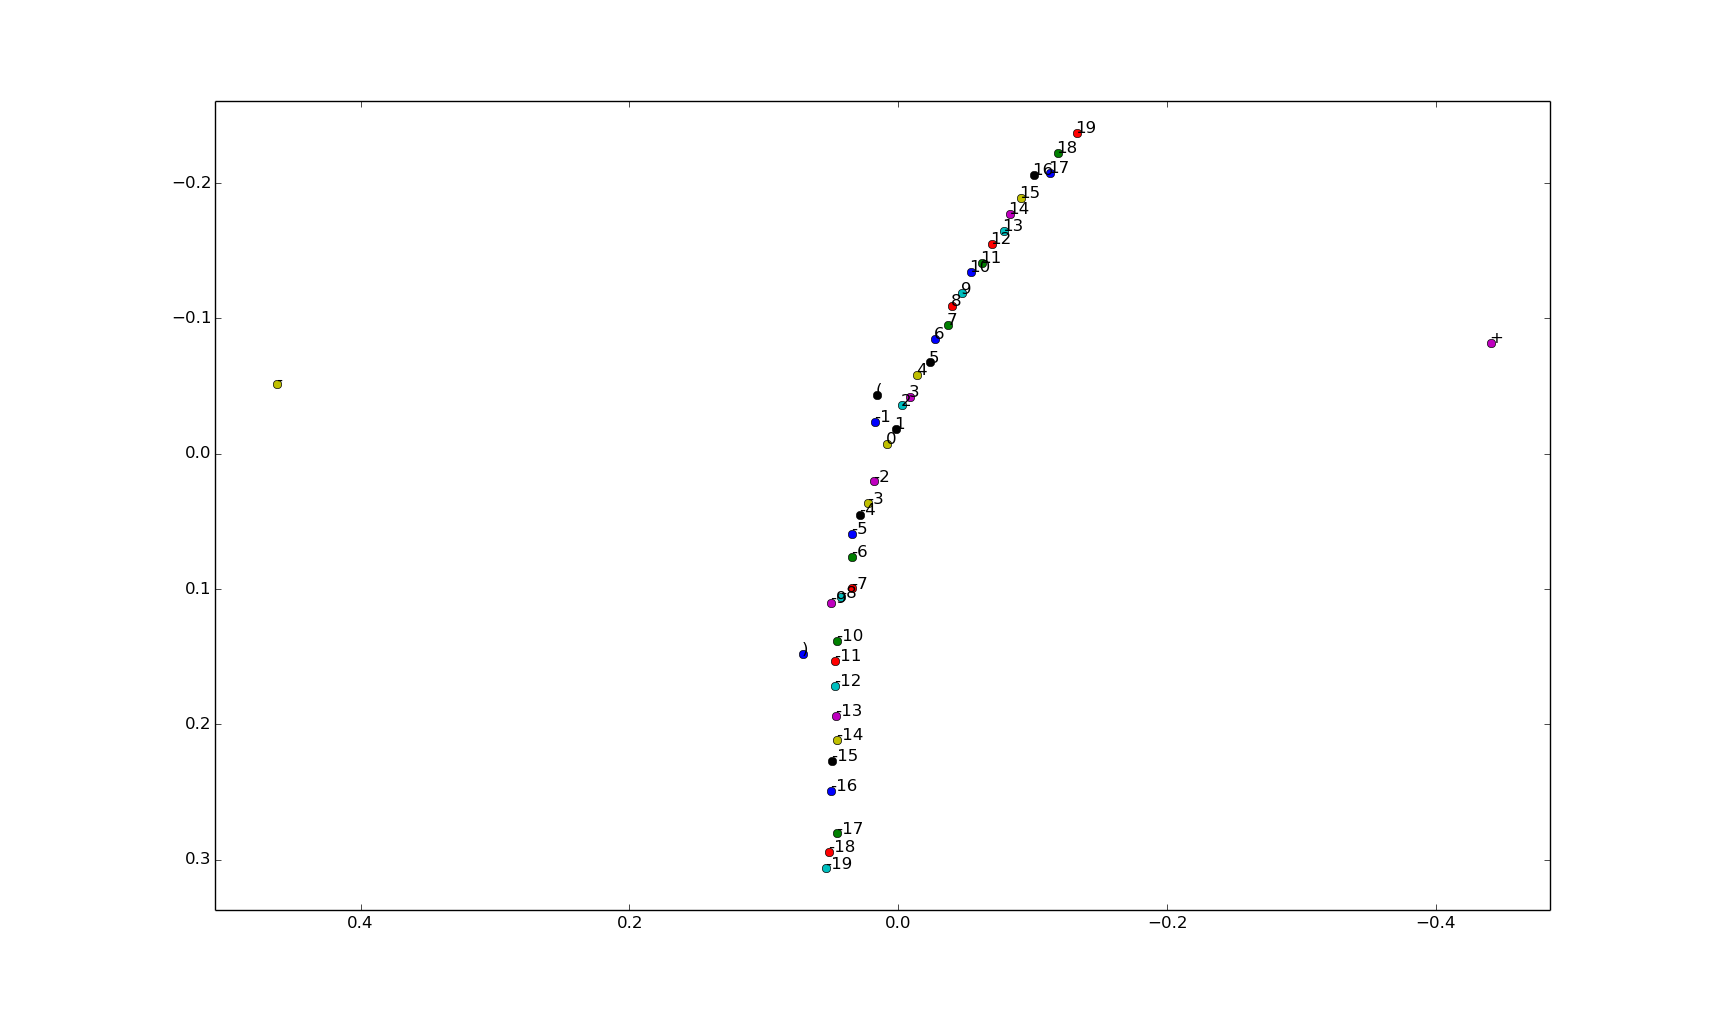
\includegraphics[scale=0.5]{SRN_L3left.png}
%     \caption{Simple recurrent layer getraind op L3left, training error was nog tamelijk hoog (rond de 5).}
% \end{figure}
% 
\end{document}
